\documentclass[a4paper]{article}

\usepackage{graphicx}
\usepackage{float}
\usepackage{listings}
\usepackage{xcolor}
\usepackage{graphicx}
\usepackage{amsmath}
\usepackage[utf8x]{inputenc}
\usepackage{fancyhdr}
\usepackage{lastpage}
% For figures and stuff
\usepackage{graphicx, wrapfig, subcaption, setspace, booktabs}
\usepackage[T1]{fontenc}
% Change for different font sizes and families
\usepackage[font=small, labelfont=bf]{caption}
\usepackage{fourier}
\usepackage[]{microtype}
\usepackage{multirow}
\graphicspath{ {./images/} } 
\usepackage{ntheorem}
\theoremseparator{:}
\newtheorem{hyp}{Hypothesis}

\definecolor{codegreen}{rgb}{0,0.6,0}
\definecolor{codegray}{rgb}{0.5,0.5,0.5}
\definecolor{codepurple}{rgb}{0.58,0,0.82}
\definecolor{backcolour}{rgb}{0.95,0.95,0.92}

\lstdefinestyle{mystyle}{
    backgroundcolor=\color{backcolour},   
    commentstyle=\color{codegreen},
    keywordstyle=\color{magenta},
    numberstyle=\tiny\color{codegray},
    stringstyle=\color{codepurple},
    basicstyle=\ttfamily\footnotesize,
    breakatwhitespace=false,         
    breaklines=true,    captionpos=b,                    
    keepspaces=true, numbers=left,                    
    numbersep=5pt, showspaces=false,                
    showstringspaces=false, showtabs=false, tabsize=2}
\lstset{style=mystyle}



\newcommand{\HRule}[1]{\rule{\linewidth}{#1}}
\onehalfspacing
\setcounter{tocdepth}{5}
\setcounter{secnumdepth}{5}

\usepackage[a4paper,top=2.5cm,bottom=2cm,left=2.5cm,right=2.5cm,marginparwidth=1.8cm]{geometry}
\pagestyle{fancy}


\setlength\headheight{15pt}
\fancyhead[L]{} 
\fancyhead[R]{}

\linespread{1.6}

%-----------------------------------------BEGIN DOC----------------------------------------
\begin{document}

\title{{\Huge \textbf{Empirical Project}{\large\linebreak\\}}{\Large \textit{The Presidential Puzzle: the continuum}\linebreak\linebreak}}

\author{Hanshuo Ma
\\ \\ \\
\textbf{University of Toronto Missisauga} \\
Department of Mathematical \& Computational Sciences \\ \\
Harry G.G. Burke \\
ECO421 \\ \\}
\date{\today}

\maketitle

\newpage
%-----------------------------------------CONTENT-------------------------------------
\tableofcontents\label{c}
\newpage

%--------------------------------------Introduction---------------------------------
\section{Introduction} \label{Introduction} 
\vspace{-10pt}

  \hspace{12pt} During the semester we've discussed market micro-structure and its inherited inefficiency and irrationality, many economists and researchers in finance  are trying to find and justify these inefficiencies to gain a better understanding of the market. One of the meaningful discussions we came across is the Presidential Puzzle - there is empirical evidence to suggest that the excess return of the stock market was higher during the years of the democratic party compared to the years of the republican party\footnote{
  Santa-Clara, P., \& Valkanov, R. (2003). The Presidential Puzzle: Political Cycles and the Stock Market. The Journal of Finance (New York), 58(5), 1841–1872. https://doi.org/10.1111/1540-6261.00590}.

  It's not entirely absurd to assume that presidents from different political parties will impose different economic policies during their term, which creates different markets based on their own political and socioeconomic beliefs. However, finding evidence that suggests regular investors can make an abnormal amount of return under the democratic party contradicts the beliefs of the efficient market hypothesis. After all, presidential election results are public information, and using that public information to obtain abnormal returns violates the semi-strong form efficiency.
  
  The study meets its fair share of criticism. Firstly, there is a limited amount of historical data between 1927 to 1998, there are only 12 presidents, and there isn't enough data to argue if the impact of the president on excess stock market return is meaningful, let alone their respective party. Secondly, the data that began with the great depression in 1929 (Republican president Herbert Hoover) greatly skewed the result in favor of the Democrat party. Nearly 26 years later, as a continuation of the study, we have included more data, and most importantly, include 2 more major financial crises. Not only do the events from the 2008 credit crisis and COVID-19 greatly improve our insight into the presidential puzzle, but the volatility of the markets on both ends of the timeline also greatly improve the density distribution of the monthly excess return data. 
  
  
\vspace{-10pt}
\section{Literature review and stating Hypothesis}\label{Review and Hypothesis}
\vspace{-10pt}
\subsection{Inspecting the Data Set} \label{Inspecting the Data Set}
\vspace{-5pt}

  \hspace{12pt} A total of three data sets are used for this analysis. The first is the monthly rate of return of the 3-Month Treasury Bill Secondary Market Rate\footnote{https://fred.stlouisfed.org/series/TB3MS} - \textbf{3MTB}. The following two are CRSP historical U.S. stock indices \footnote{CRSP US STOCK \& INDEXES, INDO: 1000510, 1000511}, the monthly rate of return for CRSP Value-Weighted Portfolios of the S\&P 500 Universe - \textbf{VWP}, and CRSP Equal-Weighted Portfolios of the S\&P 500 Universe - \textbf{EWP}. The last two are the monthly excess returns of the previous two portfolios compared to the benchmark - the 3-Month Treasury Bill rate, $\textbf{Value Excess} = VWP - 3MTB$, and $\textbf{Equal Excess} = EWP - 3MTB$. All these data sets contain data between January 1934 and December 2023, each date also references a dummy variable - the democratic party represented by 0, and the republican party represented by 1. 
  Here are the first 10 observations from the data set in \textbf{Table 1}.

  In total, we have 1079 observations, as a statistician the sample size does bring a smile to my face, with such a large sample size, the Central Limit Theorem applies, and a normal approximation is accurate. When we look at our data in  \textbf{Figure 1}, it's not surprising that our value-weighted portfolio and equal-weighted portfolio behave almost the same, and have very similar expected returns; considering S\&P500 has a very diversified stock selection, and it a huge basket, the difference in the monthly rate of return in 90 years can be negligible. However, we can still see there's a tiny bit of an increase in volatility in value-weighted portfolios through tout the years.
  
\begin{figure}[t]
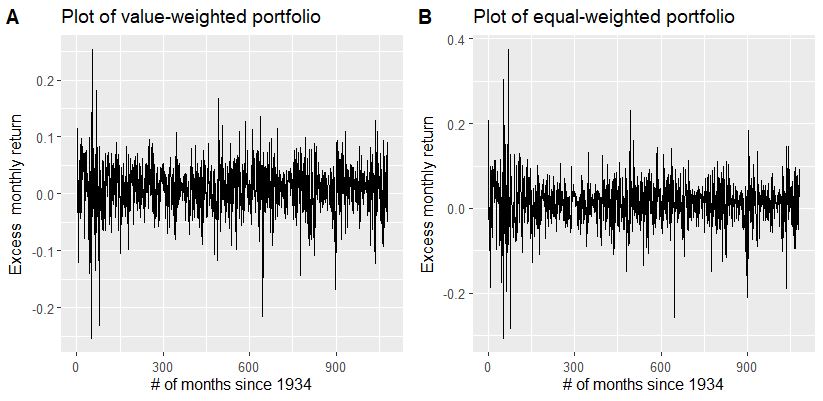
\includegraphics[scale=0.75]{images/ECO421_Plot1.png}
\caption{Comparison between value-weighted and equal-weighted portfolios}
\end{figure}

\begin{table}[H]
\begin{tabular}{ |p{1.5cm}||p{2cm}|p{2cm}|p{2cm}|p{2cm}|p{2cm}|p{0.8cm}|}
 \hline
 \multicolumn{7}{|c|}{1934-2023 Monthly excess return} \\
 \hline
Date & 3MTB & VWP & EWP & Value Excess & Equal Excess & Party\\

 \hline
 1934-01 & -0.1495 & -0.0328 & -0.0269 & 0.1167      & 0.1226 & 0 \\
 \hline
 1934-02 & -0.9491 & 0.0054 & 0.0021 & 0.9544  & 0.9512   & 0 \\
  \hline
 1934-03 & -0.4700 & -0.0255 & -0.0088 & 0.4445  & 0.4612    & 0 \\
  \hline
 1934-04 & 0.0645  & -0.0785 & -0.0999 & -0.1430  & -0.1644   & 0 \\
  \hline
 1934-05 & -0.0645  & 0.0241 & 0.0272 & 0.0886  & 0.0917   & 0 \\
  \hline
 1934-06 & 0.0000  & -0.1198 & -0.1876 & -0.1198 & -0.1876   & 0 \\
  \hline
 1934-07 & 0.2364 & 0.0586 & 0.0982 & -0.1777 & -0.1382   & 0 \\
  \hline
 1934-08 & 0.1001 & -0.0002 & 0.0050 & -0.1003 & -0.0951    & 0 \\
  \hline
 1934-09 & 0.2513 & -0.0327 & -0.0442 & -0.2840 & -0.2955   & 0 \\
  \hline
 1934-10 & 0.0770 & 0.0861 & 0.0894 & 0.1630 & 0.1663     & 0 \\
 \hline
\end{tabular}
\caption{First 10 observations from the data set}
\end{table}



\begin{figure}[t]
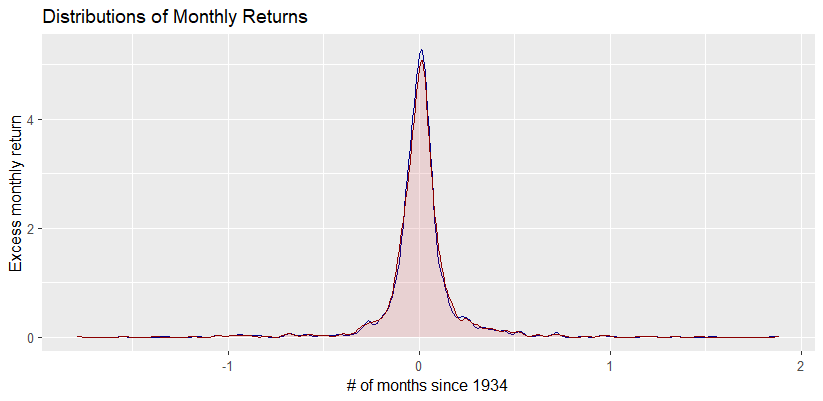
\includegraphics[scale=0.60]{images/ECO421_Plot2.png}
\caption{Comparison between value-weighted and equal-weighted portfolios}
\end{figure}

Since the Central Limit Theorem applies, we can plot the density distribution of the monthly excess return for both portfolios in \textbf{Figure 2}. We can see that, our observation was indeed, correct. Both portfolios exhibit returns that follow a normal distribution, and the value-weighted portfolio's bell shape is slightly slender and taller than equal-weighted portfolios, and it also has more outliers in its density distribution. One interesting note, both density distributions look like normal distributions sitting around $\mu = 0$, this in itself supports the efficient market hypothesis, where in the long-term, most investors make an average of abnormal excess return of zero. 

\begin{figure}[t]
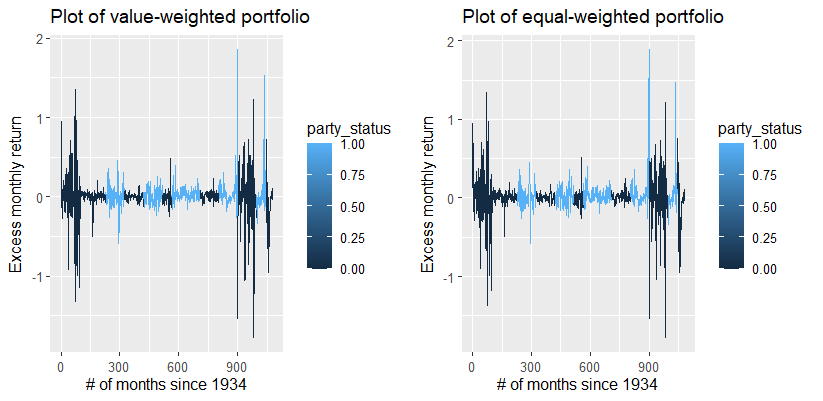
\includegraphics[scale=0.80]{images/ECO421_Plot3.png}
\caption{Comparison between value-weighted and equal-weighted portfolios, Republican = 1, Democrat = 0}
\end{figure}


Now move on to the star of the show: how do both \textbf{Value Excess} and \textbf{Equal Excess} portfolio's monthly excess return behave under two different parties? And if such a difference exists, can we show the statistical significance of such result? We can't answer the second part of the question yet, however, as we can observe in \textbf{Figure 3}. We noticed that, despite both parties having dramatic volatility changes on multiple occasions, the republican party seems to have more sudden increases in monthly excess return than the Democrats, especially right before the 2008 credit crisis, and the COVID-19 stock market crash. On average, the republican party has far less change in volatility of the monthly excess return, only a handful of the change of monthly excess returns exceed 0.5\%.

\subsection{Main Hypotheses} \label{Main Hypotheses}

\hspace{12pt} With a better visualization of the dataset we're working with, now it's time to propose our main hypothesis and answer them with respective analyses. Using the model from the original study, we have: 
$$
r_{i} = \beta_{0i} +\beta_{i1}\pi_{i} + \epsilon_{i}, \text{       
     }
\mathbb \pi(x) = 
\begin{cases}
1\hspace{0.5cm} \text{if } x\in \text{Republican}\\
0\hspace{0.5cm} \text{if } x\in \text{Democrat}
\end{cases}
$$

$r_{i}$ represents the monthly excess return, and $\pi$ represents the dummy variable of the respective party of the president and $\epsilon \in N(0, 1)$ We construct a system of linear equations for both portfolios using OLS estimators. \\
\\

\begin{hyp}[H\ref{hyp:first}] \label{hyp:first}
The market is efficient in the long term (no abnormal return on average): 
\end{hyp} $H_{o}: \mu_\text{Value Excess} = \mu_\text{Equal Excess} = 0$

\begin{hyp}[H\ref{hyp:second}]The Value-weighted portfolio's excess returns are the same under the Democrat and the Republican party. \label{hyp:second}
\end{hyp} $H_{o}: \mu_{\pi = 0, \text{Value Excess}} = \mu_{\pi = 1,\text{Value Excess}} = 0$

\begin{hyp}[H\ref{hyp:third}]The Equal-weighted portfolio's excess returns are the same under the Democrat and the Republican  party. \label{hyp:third}
\end{hyp} $H_{o}: \mu_{\pi = 0, \text{Equal Excess}} = \mu_{\pi = 1,\text{Equal Excess}} = 0$

\begin{hyp}[H\ref{hyp:fourth}] \label{hyp:fourth}
The time series process of monthly excess return under the Republican party is the same as the monthly excess return under the Democrat party. 
\end{hyp} $H_0: \text{ARIMA Models are the same}$

\begin{hyp}[H\ref{hyp:fifth}] \label{hyp:fifth}
The OLS regression coefficient of monthly excess return under the Republican party is the same as the monthly excess return under the Democrat party. 
\end{hyp} $H_0: \beta_{1, \pi = 0} = \beta_{1, \pi=1} = 0$

\begin{figure}[t]
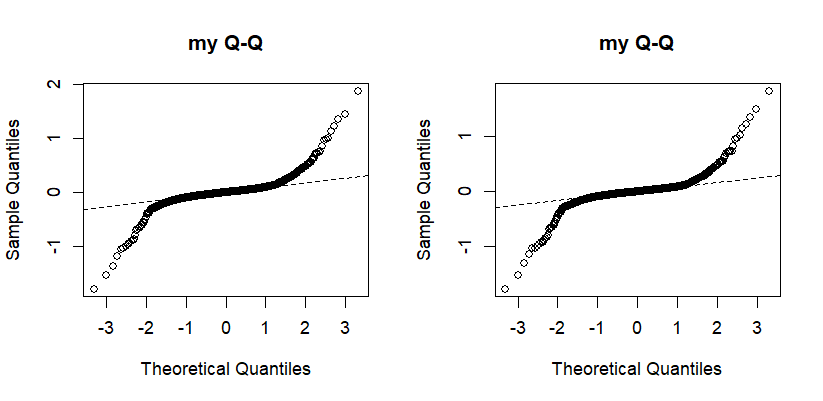
\includegraphics[scale=0.80]{images/ECO421_Plot4.png}
\caption{Q-Q plots of both Equal and Value Excess}
\end{figure}

\section{Methodology}\label{Methodology}
\vspace{-10pt}
\subsection{OLS assumptions}
\vspace{-10pt}
    \hspace{12pt} Using Q-Q plots in \textbf{Figure 4}, we can be certain the data satisfies all OLS assumptions. Thus, we could do regression analysis on the impact of political party within the monthly excess return on both Equal-Weighted and Value-Weighted portfolios.
    
    \textbf{MLR.1: } Linear in Parameters is satisfied with our model in population.

    \textbf{MLR.2: } Random Sampling is not satisfied, however, because of our large sample size, the Central Limit Theorem compensates for this drawback. 

    \textbf{MLR.3: } No Perfect Collinearity is satisfied since we only have one explanatory variable. 

    \textbf{MLR.4: } Zero Conditional Mean is satisfied by the model's construction. 

    \textbf{MLR.5: } Homoskedasticity is satisfied.

    \textbf{MLR.6: } The normality assumption of unobservable holds by the model's construction. 
\vspace{-10pt}
\subsection{Two-sample T-test}
\vspace{-10pt}
\hspace{12pt} Considering both Equal-Weighted and Value-Weighted portfolios' monthly excess returns are approximately normally distributed, and we saw in the density graph both distributions have equal variance, we can use a Two-sample t-test to determine if there's a significant difference between the means of Equal-weighted excess return and Value-weighted excess return. Not only that we can use it to determine the difference between the Republican's equal excess and the Democrat's equal excess. 

\vspace{-10pt}
\subsection{ANOVA}
\vspace{-10pt}

\hspace{12pt} We may also use ANOVA to achieve the same purpose as the above two-sample t-test. Instead of t-test statistics, we would calculate F-test statistics. 

\vspace{-10pt}
\subsection{Time Series Analysis}
\vspace{-10pt}
\hspace{12pt} Find ARIMA$(p, d, q)$ models of the time series process of Equal-Weighted and Value-Weighted portfolios' monthly excess returns of both parties. Then, compare if they are indeed the same time series process, thus we can conclude if the political parties impact on U.S. stock monthly excess returns. 

\textbf{Stationarity: A Stationary series is one whose statistical properties, such as mean, variance, and covariance, do not vary with time.} If the time series process are non-stationary, we will need to differentiate the time series to convert them into a stationary time series for analysis, use $d$ to represent the number of times the time series have been differentiated. 

\textbf{Auto regressive process, AR(p):} Current value depends linearly on its own previous values


\textbf{Moving Average process, MA(q):} Current value depends linearly on its previous error values (white noise) that are independent from the time series process. 



%-----------------------------------------Conclusion-----------------------------------
% \textcolor{red}{(I don't think we varied the temperature enough - Lucas)}
\section{Conclusion and Limititaion} \label{Conclusion}

\vspace{-10pt}
\subsection{Two-Sample T-test}\label{Results}
\vspace{-10pt}
\hspace{12pt}
    \textbf{H1:} The test statistics are $t = 0.15674, p = 0.8755$, they are \textbf{NOT} statistically significant, we fail to reject the null hypothesis. This result does support the efficient market hypothesis. In the long term, despite different portfolio structures and risk profiles in the stock market, investors on average make an abnormal excess return of zero. 

    \textbf{H2:} The test statistics are $t = 2.3343, p = 0.01976$, they are statistically significant at 5\% significance level, we reject the null hypothesis. The mean of Value-weighted portfolio excess return is higher under the Republican party than under the Democrat party.

    \textbf{H3:} The test statistics are $t = 2.4418, p= 0.01477$, they are statistically significant at 5\% significance level, we reject the null hypothesis. The mean of Equal-weighted portfolio excess return is higher under the Republican party than under the Democrat party.

    \textbf{Conclusion for the main hypotheses H1, H2, and H3:} On average, the average investors will be able to gain higher monthly excess return in the stock market under the Republican party than Democrat party.  

\vspace{-10pt}
\subsection{ANOVA}\label{Results}
\vspace{-20pt} 
\hspace{12pt}

We can verify \textbf{H2} using ANOVA table: 
\begin{center}
\begin{tabular}{||c c c c c||} 
 \hline
 DF & Sum Sq & Mean Sq & F value & Pr(>F) \\ [0.5ex] 
 \hline\hline
 1 &  0.30  & 0.30327    & 5.963 & 0.0148  \\ 
 \hline
 1077   & 54.78  & 0.05086 & & \\
 \hline
 

\end{tabular}
\end{center}

We can verify \textbf{H3} using ANOVA table: 
\begin{center}
\begin{tabular}{||c c c c c||} 
 \hline
 DF & Sum Sq & Mean Sq & F value & Pr(>F) \\ [0.5ex] 
 \hline\hline
 1 &  0.28 & 0.28049 & 5.449 & 0.0198  \\ 
 \hline
 1077   & 55.44  & 0.05147 & & \\
 \hline
 

\end{tabular}
\end{center}

\vspace{-10pt}
\subsection{OLS Results}\label{Results}
\vspace{-10pt}
\hspace{12pt}  Using OLS estimator we obtained the following results for Value-Weighted portfolio: 

\begin{center}
\begin{tabular}{||c c c c c||} 
 \hline
  & Estimate & Std. Error & t value & Pr(>|t|) \\ [0.5ex] 
 \hline\hline
 (Intercept) &  -0.0072 & 0.0092 & -0.781 & 0.4349  \\ 
 \hline
 Republican   & 0.0337  & 0.0138 &  2.442 &  0.0148 \\
 \hline

\end{tabular}
\end{center}

Using OLS estimator we obtained the following results for Equal-Weighted portfolio: 

\begin{center}
\begin{tabular}{||c c c c c||} 
 \hline
  & Estimate & Std. Error & t value & Pr(>|t|) \\ [0.5ex] 
 \hline\hline
 (Intercept) &  -0.0051 & 0.0093 & -0.550 & 0.5828  \\ 
 \hline
 Republican   & 0.0324  & 0.0139 &  2.334 & 0.0198 \\
 \hline

\end{tabular}
\end{center}

Our conclusion for the main hypothesis \textbf{H5} are based on the t-value for both portfolio's explanatory variable.The t-test statistics suggest that at a 5\% significance level, we reject our null hypothesis. Not only there's a difference to the monthly excess return of both portfolio under the republican party, on average, the average investors make as much as 3\% monthly excess return in the stock market, under the republican party. Under democratic party, on average, the average investors make -0.7\% and -0.5\% monthly excess return in the stock market on Value-weighted and Equal-weighted portfolios, respectively. 


\vspace{-10pt}
\subsection{Time Series analysis}\label{Results}
\vspace{-10pt} 
\hspace{12pt} We use the Augmented Dickey-Fuller Test to determine if our time series data is stationary, or not. By using the test-statistics and its respective p-value we can see that all four time series are stationary. We can interpret it as, in the long term, the market behaviour doesn't change depending on the time, allow us to estimate its behavior more accuarately. 

\begin{center}
\begin{tabular}{||c | c c ||} 
 \hline
 ADF p-value & Value Excess & Equal Excess \\ [0.5ex] 
 \hline\hline
 Democrat &  $<$ 0.01 & $<$ 0.01  \\ 
 \hline
 Republican   & $<$ 0.01  & $<$ 0.01  \\
 \hline
 

\end{tabular}
\end{center}


Overall, our estimated ARIMA mode with their respective order is: 

\begin{center}
\begin{tabular}{||c | c c ||} 
 \hline
  ARIMA(p,d,q) & Value Excess & Equal Excess \\ [0.5ex] 
 \hline\hline
 Democrat &  ARIMA(3,0,1) & ARIMA(3,0,1)  \\ 
 \hline
 Republican   & ARIMA(0,0,2) & ARIMA(0,0,2) \\
 \hline
 
\end{tabular}
\end{center}

We can see that, if we treat the monthly excess return of both Value-weighted and Equal-weighted portfolios under Republican and Democrat parties as two \textbf{continuous and separate} time series, they exhibits different properties as shown in their respective ARIMA model. Under the Republican party, the time series are moving average processes, MA(2), which is always stationary. In other word, the current month excess rate most likely to depend on the past 2 month's random shock under the Republican party.

\vspace{-10pt}
\subsection{Overall Conclusion}
\vspace{-10pt}
\hspace{12pt} Firstly, we find evidence to suggest that, in the long term, the average of
monthly excess return of Equal-weighted and Value-weighted portfolios are zero. Secondly, we find evidence to suggest that in the long term, the average of monthly excess return of both portfolios are higher under Republican party than it was under Democrat party. Thirdly, in the long term, the time series process of monthly excess return of both portfolios behave as MA(2) process under the Republican party, and ARMA(3,1) process under the Democrat party.

There are fair amount of evidence to suggest the monthly excess return behave differently under Republican party and Democrat party, and the average investors would be making a 3\% more monthly excess return, on average, under the Republican party. However this correlation doesn't translate into causation. To determine if this is a coincidence or compelling evidence, the study requires a deeper analysis with more explanatory variables included. 

Finally, the data seems to support the efficient market hypothesis. In the long term, regardless of portfolio risk profile and stocks' weighting in the portfolio, a diversified portfolio on average, generate a monthly excess return of zero. 

\subsection{Limitation}
\vspace{-10pt}
\subsubsection{Potential Omitted Variable Bias}
\label{Omitted Variable Bias}
\vspace{-10pt}
 \hspace{12pt} Many other factors have a concrete impact on the stock market's performance, such as interest rate, inflation, unemployment rate, fiscal policy, trade policy, etc. Not including those variables in our regression analysis may include potential bias in our results. Many global events have increased the change in volatility in the unpredictable market, and to say that the unexpected swing in profitability is due to the president's own party's agenda rather than luck is absurd. 

\vspace{-10pt}
\subsubsection{Core issues with the data}
\label{Core issues with the data}
\vspace{-10pt}
 \hspace{12pt}
 The core critism of the data still persist - we still have a relatively small sample of presidents to determine if their parties' responsible for performance of the stock market and the economy as whole. Especially when major macroeconomic monetary policy - interest rate, only played an important role in our modern economy less than 100 years.  To expan upon the presidential puzzle, conservatively speaking, we need to wait at least another 100 years to even have a workable sample size.
 
 \vspace{-10pt}
\subsubsection{Historical data} 
\label{Historical data} 
\vspace{-10pt}
 \hspace{12pt} It's been discussed and debated over many years, and the geniue consensus is that, it's simply not possible to use historical data to predict the future. The market is unpredictable and there are little information about the future we can extract using historical data. Here we also have a problem that historically Democract party have more observations than the republican party, and this larger frequency may be the reason monthly excess return were closer to zero expected return than the republican party.  

\newpage
\appendix
\section{R code}

\begin{lstlisting}[language=R]
library(ggplot2)
library(ggpubr)
library(dplyr)
library(lme4)
library(tseries)
library(forecast)

# Value-weighted portfolio 
value_data <- read.csv("Value_weighted.csv")
# Equal-weighted portfolio 
equal_data <- read.csv("Equal_weighted.csv")
# Three month T-bill Rate 
TB3MS <- read.csv("TB3MS.csv")
# president data republican = 1, democrat = 0
president_data <- read.csv("Presidential_Party_by_Month.csv")
party_status <- president_data$Party[2:1080]
T_bill <- TB3MS$TB3MS


one <- ggplot(TB3MS, aes(x=seq(1,1080), y=TB3MS))+
  geom_line() +
  
  labs(title="Plot of average excess equal-weighted monthly return",
       x ="# of months since 1934", y = "Excess Equal-Weighted monthly return" 
  )
two <- ggplot(value_data, aes(x=seq(1,1080), y=COL1))+
  geom_line() + labs(title="Plot of value-weighted portfolio",
                     x ="# of months since 1934", y = "Excess  monthly return")

three <- ggplot(equal_data, aes(x=seq(1,1080), y=COL1))+
  geom_line() + labs(title="Plot of equal-weighted portfolio",
                     x ="# of months since 1934", y = "Excess monthly return")

example <- ggarrange(two,
                    three,
                    ncol = 2,
                    nrow = 1,
                    # First row with line plot
                    labels = c("A","B") # Label of the line plot
)

example


x <- seq(1, 1079);
T_df <- data.frame(T_bill);
n <- nrow(T_df)
ccret <- log(T_df[2:n, 1]) - log(T_df[1:(n-1), 1])
ccret_df <- data.frame(ccret)

T_mreturn <- ccret_df$ccret
# Excluding first month, because it is unobtainable 
# from the T-bill data. 
v_return <- value_data$COL1[2:1080]
e_return <- equal_data$COL1[2:1080]

V_T <-  v_return-T_mreturn
E_T <- e_return - T_mreturn

df_combined <- data.frame(T_mreturn, v_return, e_return, V_T, E_T, party_status)
democrat_data <- df_combined %>% filter(party_status == 0)
republican_data <- df_combined %>% filter(party_status == 1)


ap <- ggplot(df_combined, aes(x = seq(1,1079), y = V_T)) + 
  geom_line(aes(color = party_status, group = 1))+
  labs(title="Plot of value-weighted portfolio",
       x ="# of months since 1934", y = "Excess monthly return" 
  )


bp <- ggplot(df_combined, aes(x = seq(1,1079), y = E_T)) + 
  geom_line(aes(color = party_status, group = 1)) + 
  labs(title="Plot of equal-weighted portfolio",
       x ="# of months since 1934", y = "Excess monthly return" 
       )


cp <- ggplot() + 
  geom_density(df_combined, mapping = aes(x = V_T), color="darkblue", fill="lightblue", alpha=0.1) +
  geom_density(df_combined, mapping = aes(x = E_T), color="darkred", fill="red", alpha=0.1) +
  labs(title="Plot of both portfolios",
       x ="# of months since 1934", y = "Excess monthly return" 
  ) + 
  ggtitle("Distributions of Monthly Log Returns")


figure <- ggarrange(ap,
                    bp,
                    ncol = 2,
                    nrow = 1
)

figure
cp

# Compute t-test
res_1 <- t.test(df_combined$V_T, df_combined$E_T, var.equal = TRUE)
res_1

res_2 <- t.test(republican_data$V_T, democrat_data$V_T, var.equal = TRUE)
res_2


res_3 <- t.test(democrat_data$E_T, republican_data$E_T, var.equal = TRUE)
res_3

lm_value_weighted <- lm(E_T ~ party_status, data = df_combined)
summary(lm_value_weighted)

q1 = qqnorm(lm_value_weighted$residuals, main = "my Q-Q"); qqline(lm_value_weighted$residuals, lty = 2)

lm_equal_weighted <- lm(V_T ~ party_status, data = df_combined)
summary(lm_equal_weighted)

q2 = qqnorm(lm_equal_weighted$residuals, main = "my Q-Q"); qqline(lm_equal_weighted$residuals, lty = 2)

par(mfrow=c(1,2))
q1
q2

e_anova = aov(E_T ~ party_status, data = df_combined)
summary(e_anova)

v_anova = aov(V_T ~ party_status, data = df_combined)
summary(v_anova)


adf.test(df_combined$E_T)
adf.test(df_combined$V_T)
adf.test(democrat_data$E_T)
adf.test(democrat_data$V_T)
adf.test(republican_data$E_T)
adf.test(republican_data$V_T)

acf(democrat_data$E_T)
pacf(democrat_data$E_T)

acf(republican_data$E_T)
pacf(republican_data$E_T)

arima_d = auto.arima(democrat_data$E_T, d = 0, max.p = 3, max.q = 3, seasonal = T)
summary(arima_d)
checkresiduals(arima_d)
tsdiag(arima_d)

arima_r = auto.arima(republican_data$E_T, d = 0, max.p = 3, max.q = 3, seasonal = T)
summary(arima_r)
checkresiduals(arima_r)
tsdiag(arima_r)


arima_d = auto.arima(democrat_data$V_T, d = 0, max.p = 3, max.q = 3, seasonal = T)
summary(arima_d)
checkresiduals(arima_d)
tsdiag(arima_d)

arima_r = auto.arima(republican_data$V_T, d = 0, max.p = 3, max.q = 3, seasonal = T)
summary(arima_r)
checkresiduals(arima_r)
tsdiag(arima_r)

\end{lstlisting}


\end{document}
